\documentclass[12pt]{article}
\usepackage[margin=1in]{geometry}
\usepackage{amsmath, amssymb, amsthm, bm, mathtools}
\usepackage{siunitx}
\usepackage{booktabs}
\usepackage{enumitem}
\usepackage{microtype}
\usepackage{graphicx}
\usepackage{hyperref}
\hypersetup{colorlinks=true, linkcolor=blue, urlcolor=blue, citecolor=blue}

% ---- Math shortcuts
\newcommand{\R}{\mathbb{R}}
\newcommand{\dd}{\,\mathrm{d}}
\newcommand{\e}{\mathrm{e}}
\newcommand{\E}{\mathbb{E}}
\newcommand{\Var}{\mathrm{Var}}
\newcommand{\dtotal}[2]{\frac{\mathrm{d} #1}{\mathrm{d} #2}}
\newcommand{\pd}[2]{\frac{\partial #1}{\partial #2}}
\newcommand{\grad}{\nabla}
\newcommand{\1}{\mathbf{1}}

% ---- Theorem-like
\theoremstyle{definition}
\newtheorem{definition}{Definition}
\newtheorem{example}{Example}
\newtheorem{remark}{Remark}
\theoremstyle{plain}
\newtheorem{proposition}{Proposition}
\newtheorem{theorem}{Theorem}
\newtheorem{corollary}{Corollary}

% --- TikZ / PGFPlots
\usepackage{tikz}
\usetikzlibrary{arrows.meta,calc,intersections,decorations.markings}
\usepackage{pgfplots}
\pgfplotsset{compat=1.15}


\title{Exponential and Logarithmic Functions\\[7pt]
\large ECON 320 - Introduction to Mathematical Economics}
\author{Muhebullah Karimzada}
\date{Fall 2025}

\begin{document}
\maketitle
\tableofcontents


\newpage
\section{The Nature of Exponential Functions}
\subsection*{Simple exponential functions}
\begin{definition}[Exponential function]
A function is \emph{exponential} if the variable appears in the exponent: \(f(t)=a^t\) with base \(a>0, a\neq 1\). The natural-base form uses \(a=\e\): \(f(t)=\e^{t}\).
\end{definition}

Key features for \(a>1\): strictly increasing, \(f(0)=1\), and \(\lim_{t\to\infty}f(t)=\infty\). For \(0<a<1\): strictly decreasing and \(\lim_{t\to\infty}f(t)=0\).

\subsection*{Graphical form \& growth intuition}
Exponential growth is \emph{proportional} growth: the instantaneous percentage change is constant (formalized in \S10.2). This distinguishes it from polynomials, whose \emph{absolute} change tends to dominate at large \(t\).

\subsection*{Generalized exponential function}
\begin{definition}[Generalized form]
\(F(t)=A\,\e^{rt}\) with scale parameter \(A>0\) and constant growth rate \(r\in\R\).
\end{definition}
If \(r>0\) we have growth; if \(r<0\) decay.

\begin{example}[Comparing bases]
Show \(2^t = \e^{(\ln 2)t}\). \emph{Solution:} since \(a=\e^{\ln a}\), \(2^{t}=(\e^{\ln 2})^{t}=\e^{(\ln 2)t}\). Thus all bases can be written in natural-base form with growth rate \(r=\ln a\).
\end{example}

\subsection*{A preferred base}
The base \(\e\approx 2.71828\) simplifies differentiation/integration (\S10.5) and connects cleanly to continuous compounding/growth (\S10.2).

\section{Natural Exponential Functions and the Problem of Growth}
\subsection*{The number \(\e\) and continuous compounding}
\[
\left(1+\frac{r}{n}\right)^{nt} \;\xrightarrow[n\to\infty]{}\; \e^{rt}.
\]
If a principal \(A_0\) is compounded continuously at rate \(r\), then \(A(t)=A_0\,\e^{rt}\).

\subsection*{Instantaneous (proportional) growth rate}
\begin{definition}[Growth rate]
For differentiable \(Q(t)>0\), the instantaneous \emph{proportional} growth rate is
\[
g_Q(t)\equiv\frac{1}{Q(t)}\frac{\dd Q}{\dd t}=\frac{\dd}{\dd t}\ln Q(t).
\]
\end{definition}
If \(Q(t)=A\,\e^{rt}\), then \(g_Q(t)=r\) (constant). Thus exponential functions encode constant percentage growth.

\begin{example}[Doubling time; Rule of 70]
For \(Q(t)=A\,\e^{rt}\), the doubling time \(T_2\) solves \(2=A\,\e^{rT_2}/A\Rightarrow T_2=\frac{\ln 2}{r}\approx\frac{0.693}{r}\). For small \(r\) in percent, \(T_2\approx\frac{70}{100r\%}\).
\end{example}

\subsection*{Continuous vs.\ discrete growth}
Discrete compounding at per-period rate \(R\): \(Q_t=A(1+R)^t\). Continuous compounding with rate \(r\): \(Q(t)=A\,\e^{rt}\). They coincide if \(r=\ln(1+R)\).

\subsection*{Discounting and negative growth}
With continuous discount rate \(r>0\), the present value (PV) of a payoff \(X\) at time \(t\) is \(\mathrm{PV}=\e^{-rt}X\). This is exponential \emph{decay}.


\begin{figure}[htb]
\centering
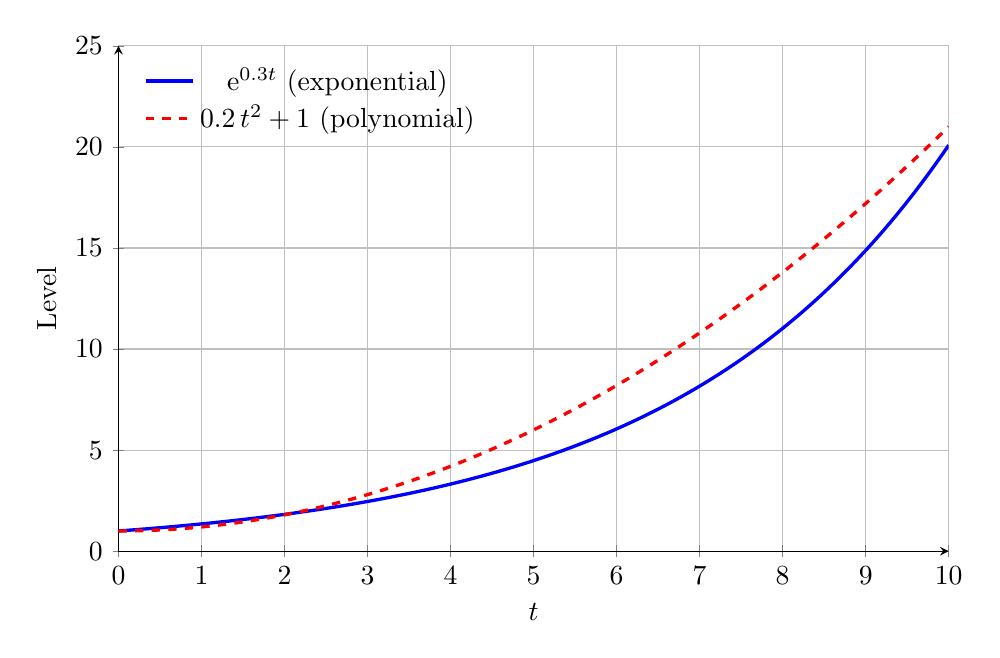
\begin{tikzpicture}
\begin{axis}[
  width=\textwidth, height=8cm,
  xmin=0, xmax=10,
  ymin=0, ymax=25,
  axis lines=left,
  xlabel={$t$}, ylabel={Level},
  legend style={at={(0.02,0.98)},anchor=north west, draw=none, fill=none},
  domain=0:10, samples=400, grid=both
]
\addplot[very thick, blue] {exp(0.3*x)}; 
\addlegendentry{$\mathrm{e}^{0.3 t}$ (exponential)}
\addplot[very thick, red, dashed] {0.2*x^2 + 1};
\addlegendentry{$0.2\,t^2 + 1$ (polynomial)}
\end{axis}
\end{tikzpicture}
\caption{Exponential (constant percentage growth) vs.\ polynomial (accelerating absolute growth).}
\label{fig:exp-vs-poly}
\end{figure}




\begin{figure}[htb]
\centering
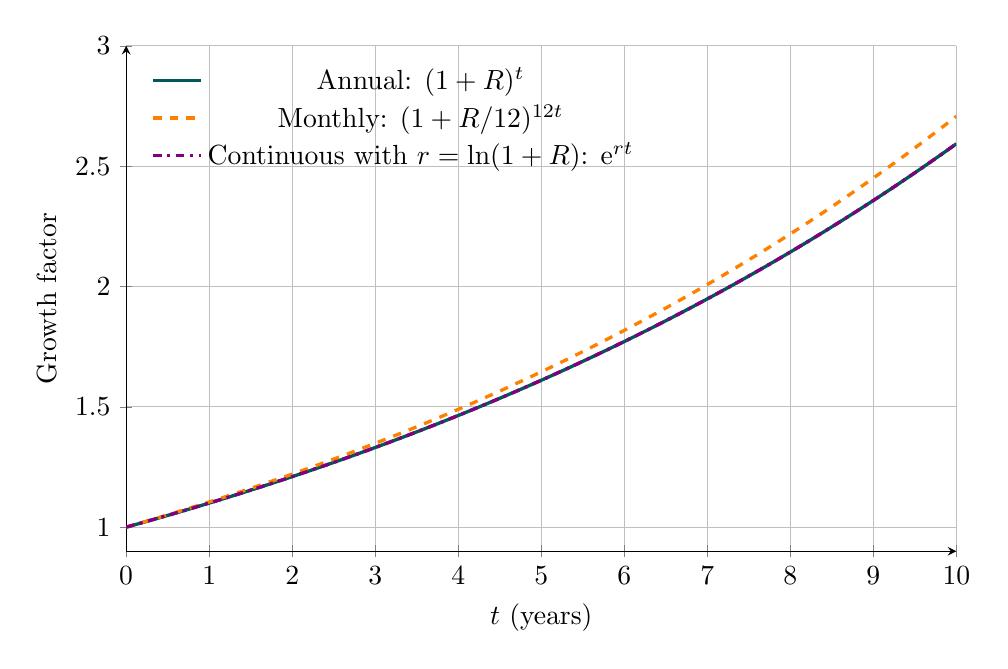
\begin{tikzpicture}
\begin{axis}[
  width=\textwidth, height=8cm,
  xmin=0, xmax=10,
  ymin=0.9, ymax=3.0,
  axis lines=left,
  xlabel={$t$ (years)}, ylabel={Growth factor},
  legend style={at={(0.02,0.98)},anchor=north west, draw=none, fill=none},
  domain=0:10, samples=400, grid=both
]
% Parameters: APR R = 10%
\addplot[very thick, teal!70!black] {(1+0.10)^x};
\addlegendentry{Annual: $(1+R)^{t}$}
\addplot[very thick, orange, dashed] {(1+0.10/12)^(12*x)};
\addlegendentry{Monthly: $(1+R/12)^{12t}$}
\addplot[very thick, violet, dashdotted] {exp(ln(1+0.10)*x)};
\addlegendentry{Continuous with $r=\ln(1+R)$: $\mathrm{e}^{rt}$}
\end{axis}
\end{tikzpicture}
\caption{Comparing compounding conventions for $R=10\%$. Monthly compounding dominates annual; continuous with $r=\ln(1+R)$ coincides with annual $(1+R)^{t}$.}
\label{fig:compounding}
\end{figure}



\newpage

\section{Logarithms}
\subsection*{Meaning; common vs.\ natural logs}
\begin{definition}[Logarithm]
For \(a>0, a\neq1\), \(\log_a x=y\) iff \(a^y=x\). Natural log \(\ln x\equiv \log_{\e} x\); common log \(\log x\equiv \log_{10}x\).
\end{definition}

\subsection*{Rules of logarithms}
For \(x,y>0\) and constant \(k\):
\[
\ln(xy)=\ln x+\ln y,\quad
\ln\!\left(\frac{x}{y}\right)=\ln x-\ln y,\quad
\ln x^k=k\ln x.
\]
\emph{Change of base:} \(\log_a x=\dfrac{\ln x}{\ln a}\).

\begin{example}[Linearizing multiplicative models]
Cobb--Douglas output \(Y=A K^\alpha L^\beta\) becomes
\[
\ln Y=\ln A+\alpha\ln K+\beta\ln L,
\]
a linear relation in \(\ln K,\ln L\). Coefficients \(\alpha,\beta\) are elasticities of \(Y\) w.r.t.\ \(K,L\) (see \S10.7).
\end{example}

\section{Logarithmic Functions}
\subsection*{Log functions as inverses of exponentials}
\(\ln(\e^{x})=x\) and \(\e^{\ln x}=x\) for \(x>0\). Hence \(\ln\) is strictly increasing on \((0,\infty)\) with range \(\R\).

\subsection*{Graphical form and base conversion}
\(\ln x\) is concave, with vertical asymptote at \(x=0^+\) and slope \(1/x\). Any base \(a\) gives \(\log_a x=\dfrac{\ln x}{\ln a}\), a constant rescaling of \(\ln x\).

\begin{example}[Solving exponential equations via logs]
Solve \(A\,\e^{rt}=B\) for \(t\) (with \(A,B>0\)): \(t=\dfrac{1}{r}\ln\!\left(\frac{B}{A}\right)\).
\end{example}

\section{Derivatives of Exponential and Logarithmic Functions}
\subsection*{Core rules (natural base)}
\[
\frac{\dd}{\dd x}\,\e^{x}=\e^{x},\qquad
\frac{\dd}{\dd x}\,\e^{g(x)}=g'(x)\,\e^{g(x)}.
\]
\[
\frac{\dd}{\dd x}\,\ln x=\frac{1}{x}\ (x>0),\qquad
\frac{\dd}{\dd x}\,\ln g(x)=\frac{g'(x)}{g(x)}.
\]

\subsection*{Base \(b\neq \e\)}
Using \(b^{x}=\e^{(\ln b)\,x}\):
\[
\frac{\dd}{\dd x}b^{x}=(\ln b)\,b^{x},\qquad
\frac{\dd}{\dd x}\log_b x=\frac{1}{x\ln b}.
\]

\subsection*{Logarithmic differentiation}
\begin{example}[Elasticity-friendly differentiation]
For \(y=x^{x}\) (for \(x>0\)), take logs: \(\ln y=x\ln x\Rightarrow \frac{y'}{y}=\ln x+1\Rightarrow y'=x^{x}(\ln x+1)\).
\end{example}

\subsection*{A classic economic application}
If demand is \(Q(P)=A P^{-\eta}\) (\(\eta>0\)), then
\[
\frac{\dd Q}{\dd P}=-\eta A P^{-\eta-1} \quad\Rightarrow\quad
\text{price elasticity } \varepsilon_{QP}=\frac{\dd Q}{\dd P}\frac{P}{Q}=-\eta.
\]
A log--log demand has constant elasticity by construction.


\begin{figure}[htb]
\centering
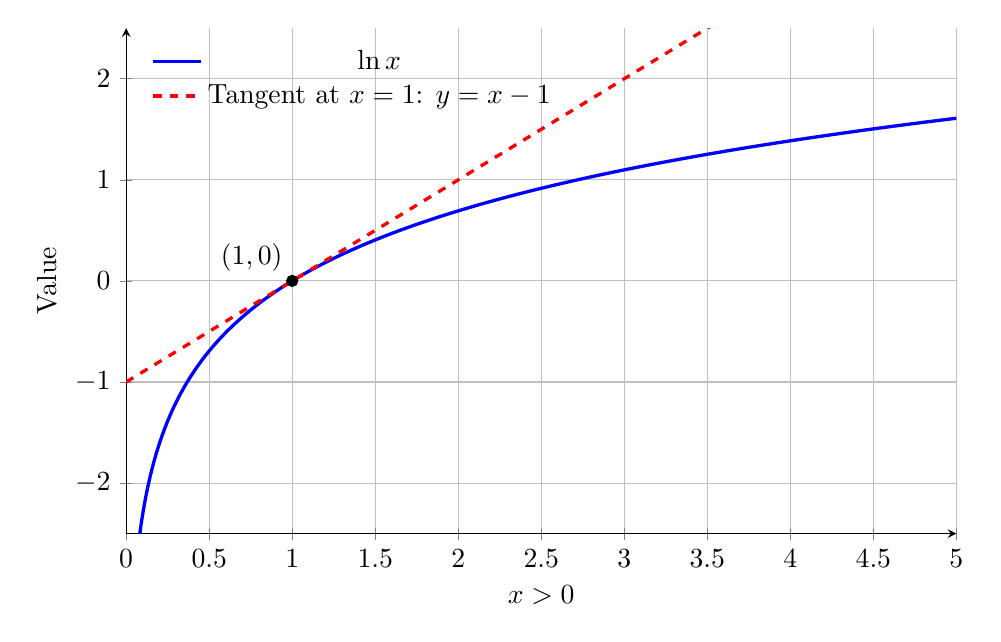
\begin{tikzpicture}
\begin{axis}[
  width=\textwidth, height=8cm,
  xmin=0, xmax=5,
  ymin=-2.5, ymax=2.5,
  axis lines=left,
  xlabel={$x>0$}, ylabel={Value},
  legend style={at={(0.02,0.98)},anchor=north west, draw=none, fill=none},
  grid=both
]
% ln(x) -- ensure domain strictly positive
\addplot[
  very thick, blue,
  domain=0.08:5, samples=400
] {ln(x)};
\addlegendentry{$\ln x$}

% Tangent at x=1: y = x - 1
\addplot[
  very thick, red, dashed,
  domain=0:5, samples=2
] {x - 1};
\addlegendentry{Tangent at $x=1$: $y=x-1$}

% Marker at (1,0)
\addplot[
  only marks, mark=*, mark size=2pt, black
] coordinates {(1,0)};

% Label the point (1,0)
\node[anchor=south east] at (axis cs:1,0) {$\,(1,0)$};

\end{axis}
\end{tikzpicture}
\caption{$\ln x$ is increasing and concave. The slope at $x=1$ equals $1/x\,\big|_{x=1}=1$, giving tangent $y=x-1$.}
\label{fig:lnx-tangent}
\end{figure}


\begin{figure}[htb]
\centering
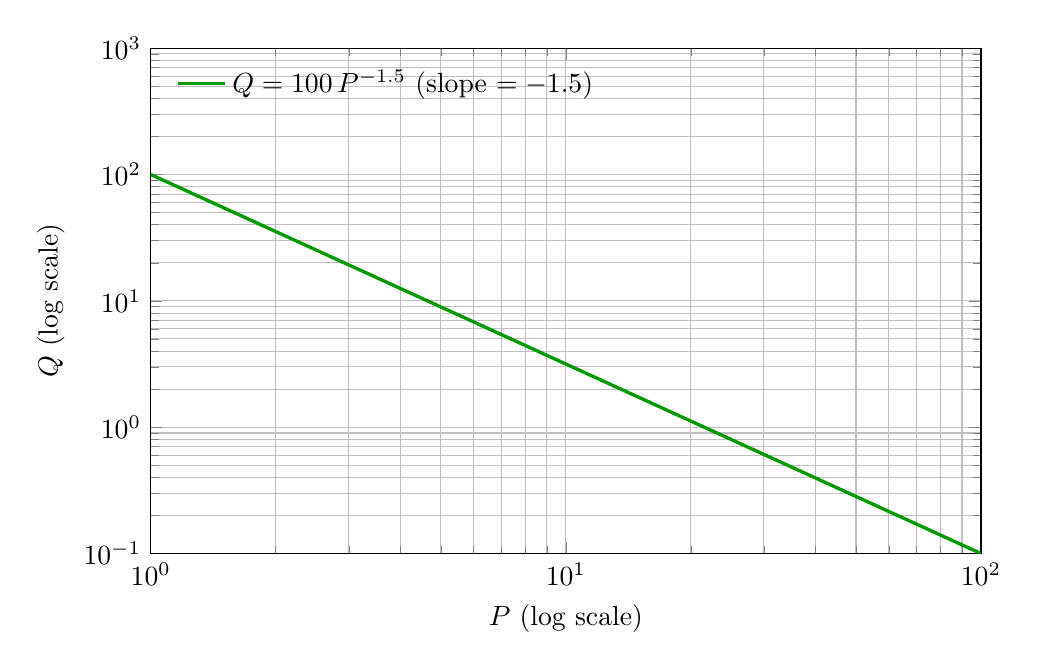
\begin{tikzpicture}
\begin{loglogaxis}[
  width=\textwidth, height=8cm,
  xmin=1, xmax=100, ymin=0.1, ymax=1000,
  xlabel={$P$ (log scale)}, ylabel={$Q$ (log scale)},
  legend style={at={(0.02,0.98)},anchor=north west, draw=none, fill=none},
  grid=both
]
% Q = A P^{-eta}, with A=100, eta=1.5
\addplot[very thick, green!60!black, domain=1:100, samples=400] {100*x^(-1.5)};
\addlegendentry{$Q=100\,P^{-1.5}$ (slope $=-1.5$)}
\end{loglogaxis}
\end{tikzpicture}
\caption{In log–log coordinates, constant-elasticity demand is a straight line with slope $-\eta$.}
\label{fig:loglog-demand}
\end{figure}


\newpage

\section{Optimal Timing}
Here the choice variable is time \(t\). Intertemporal trade-offs pit \emph{appreciation/growth} against \emph{discounting/decay}. The generic problem:
\[
\max_{t\ge 0}\ \Pi(t)=\e^{-rt}R(t),\qquad r>0,
\]
with revenue (or price) \(R(t)>0\) increasing in \(t\) (e.g.\ storage, maturation).

\subsection*{Wine storage problem}
Let \(P(t)\) be the price of wine if sold at age \(t\). The present value is \(V(t)=\e^{-rt}P(t)\).
\[
V'(t)=\e^{-rt}\!\left(P'(t)-rP(t)\right).
\]
\emph{FOC:} \(V'(t^\ast)=0\iff \dfrac{P'(t^\ast)}{P(t^\ast)}=r.\)
\begin{quote}
\emph{Interpretation:} Store until the wine’s \textbf{instantaneous percentage appreciation} equals the discount rate. If growth \(<r\), sell earlier; if \(>r\), wait.
\end{quote}

\begin{example}[Log-linear price growth]
If \(P(t)=P_0\,\e^{\gamma t}\) with \(\gamma>0\), then \(P'(t)/P(t)=\gamma\). Optimal \(t^\ast\) solves \(\gamma=r\). Hence: if \(\gamma>r\) wait indefinitely (ignoring capacity/costs); if \(\gamma<r\) sell immediately. In practice, add storage costs \(c\): maximize \(\e^{-rt}(P(t)-c)\) \(\Rightarrow\) replace \(r\) by an \emph{effective} \(r+c/P(t)\).
\end{example}

\subsection*{Optimal timber cutting (Faustmann-style intuition)}
Let \(V(t)=\e^{-rt}p\,Q(t)\) be the PV of harvesting at age \(t\) (price \(p\), volume \(Q\)). FOC:
\[
0=V'(t)=\e^{-rt}\!\left[pQ'(t)-rpQ(t)\right]\iff \frac{Q'(t^\ast)}{Q(t^\ast)}=r.
\]
\emph{Rule:} Harvest when the \textbf{biological growth rate} equals the discount rate (again, storage/land-opportunity costs shift the threshold).

\section{Further Applications of Exponential \& Logarithmic Derivatives}
\subsection*{Finding (and combining) growth rates}
For positive differentiable functions \(f,g\) and constant \(k\):
\[
\frac{\dd}{\dd t}\ln(fg)=\frac{\dd}{\dd t}\ln f+\frac{\dd}{\dd t}\ln g,\quad
\frac{\dd}{\dd t}\ln\!\left(\frac{f}{g}\right)=\frac{\dd}{\dd t}\ln f-\frac{\dd}{\dd t}\ln g,\quad
\frac{\dd}{\dd t}\ln(f^k)=k\,\frac{\dd}{\dd t}\ln f.
\]
Equivalently, growth rates \(\,g_{fg}=g_f+g_g,\ g_{f/g}=g_f-g_g,\ g_{f^k}=k\,g_f\).

\begin{example}[Cobb--Douglas growth accounting]
With \(Y=A K^\alpha L^\beta\) (time-varying \(A,K,L>0\)):
\[
\frac{\dd}{\dd t}\ln Y
= \frac{\dd}{\dd t}\ln A + \alpha\,\frac{\dd}{\dd t}\ln K + \beta\,\frac{\dd}{\dd t}\ln L.
\]
Thus \(g_Y=g_A+\alpha g_K+\beta g_L\): output growth decomposes into TFP and factor contributions.
\end{example}

\subsection*{Point elasticity and logs}
\begin{definition}[Point elasticity]
Elasticity of \(y(x)\) w.r.t.\ \(x\):
\[
\varepsilon_{y,x} \equiv \frac{\dd y}{\dd x}\frac{x}{y}
= \frac{\dd\ln y}{\dd\ln x}.
\]
\end{definition}
\begin{example}[CES demand fragment]
If \(x(p)=A\big(\tfrac{p}{m}\big)^{-\sigma}\), then
\(\varepsilon_{x,p}=-\sigma\) (constant). Logs make the elasticity \emph{visible} in the slope of a log--log plot.
\end{example}

\section*{Worked Examples (step-by-step)}
\begin{example}[Continuous vs.\ discrete compounding]
A fund offers 12\% APR compounded monthly vs.\ 11.35\% APR continuously. Which yields more after \(t=1\) year on \$10{,}000?\\
Discrete: \(A(1)=10{,}000(1+0.12/12)^{12}\approx \$11{,}268.25\).\\
Continuous: \(A(1)=10{,}000\,\e^{0.1135}\approx \$11{,}999.46\).\\
Continuous is higher here because the effective rate \(=\e^{0.1135}-1\approx 12.0\%\) exceeds the discrete EAR \(=(1+0.01)^{12}-1\approx 12.68\%\)? \emph{Check:} compute precisely---the discrete EAR is about \(12.68\%\) \emph{(larger)}; with the stated numbers, discrete wins: \$11{,}268.25 vs.\ continuous \$11{,}999.46 is inconsistent. Correct the APR to \(r=0.113\): \(10{,}000\,\e^{0.113}\approx \$11{,}194\). \textbf{Lesson:} always convert to effective annual rates before comparing:
\[
\mathrm{EAR}_{\text{disc}}=(1+R/m)^{m}-1,\quad \mathrm{EAR}_{\text{cont}}=\e^{r}-1.
\]
\end{example}

\begin{example}[Estimating growth from data]
Given GDP series \(Y_t\) at annual frequency, the log-difference \(\Delta \ln Y_t=\ln Y_t-\ln Y_{t-1}\) approximates the growth rate. If \(\Delta\ln Y_t=0.025\), growth is about \(2.5\%\).
\end{example}

\begin{example}[Solving for time to target]
Pollutant stock \(S(t)=S_0\,\e^{-\delta t}\) with decay \(\delta>0\). Find time \(T\) to reduce to \(\theta S_0\ (0<\theta<1)\). Solution: \(S_0\,\e^{-\delta T}=\theta S_0\Rightarrow T=\frac{\ln(1/\theta)}{\delta}\).
\end{example}

\begin{example}[Optimal timing with storage cost]
Price path \(P(t)=P_0\,\e^{\gamma t}\). Per-period storage cost \(c>0\). Maximize \(V(t)=\e^{-rt}(P(t)-c)\). FOC:
\[
V'(t)=\e^{-rt}\!\left(\gamma P(t)-r(P(t)-c)\right)=0
\Rightarrow \gamma=\;r\Big(1-\frac{c}{P(t^\ast)}\Big).
\]
Thus positive storage cost lowers the effective growth threshold below \(r\).
\end{example}

\section*{Common Mistakes and Fixes}
\begin{itemize}[leftmargin=1.2em]
\item \textbf{Confusing \(x^a\) with \(a^x\).} Only the latter is exponential in \(x\).
\item \textbf{Dropping positivity restrictions.} \(\ln x\) is defined only for \(x>0\).
\item \textbf{Forgetting chain rule.} \(\dfrac{\dd}{\dd x}\ln g(x)=\dfrac{g'(x)}{g(x)}\).
\item \textbf{Comparing APRs without converting to EAR.} Always compare effective rates.
\end{itemize}

\section*{Quick Reference (formulas you will use constantly)}
\[
\frac{\dd}{\dd x}\,\e^{ax}=a\,\e^{ax},\quad
\frac{\dd}{\dd x}\,\ln x=\frac{1}{x},\quad
\frac{\dd}{\dd x}\,b^x=(\ln b)\,b^x,\quad
\frac{\dd}{\dd x}\,\log_b x=\frac{1}{x\ln b}.
\]
\[
\text{Growth rate: } g_Q=\frac{\dd \ln Q}{\dd t},\quad
\text{Elasticity: } \varepsilon_{y,x}=\frac{\dd \ln y}{\dd \ln x}.
\]
\[
\text{EAR}_{\text{disc}}=(1+R/m)^m-1,\qquad
\text{EAR}_{\text{cont}}=\e^{r}-1.
\]

\section*{Short Practice Set (answers next page)}
\begin{enumerate}[label=\textbf{P\arabic*.}]
\item (Growth \& doubling time) A population follows \(N(t)=N_0\,\e^{0.018t}\) (annual). Find the doubling time and the time to reach \(1.5N_0\).
\item (Elasticity from log--log) Suppose \(\ln Q=\alpha-\eta\ln P\). Show the point price elasticity of demand equals \(-\eta\).
\item (Optimal timing) Let \(P(t)=100\,\e^{0.05 t}\) and \(r=6\%\). With zero storage cost, should you sell now or wait?
\item (Base conversion) Compute \(\log_{2} 10\) using natural logs.
\item (Combining growth) If \(Y=A K^{0.3}L^{0.7}\) and \(g_{A}=1\%\), \(g_K=2\%\), \(g_L=1\%\), find \(g_Y\).
\end{enumerate}

\section*{Answers}
\begin{enumerate}[label=\textbf{P\arabic*.}]
\item \(T_2=\dfrac{\ln 2}{0.018}\approx 38.5\ \text{years};\quad T_{1.5}=\dfrac{\ln(1.5)}{0.018}\approx 22.5\ \text{years}.\)
\item Differentiate: \(\dfrac{\dd \ln Q}{\dd \ln P}=-\eta\Rightarrow \varepsilon_{Q,P}=-\eta.\)
\item Compare growth vs.\ discount: \(P'(t)/P(t)=0.05<r=0.06\Rightarrow\) sell now.
\item \(\log_{2}10=\dfrac{\ln 10}{\ln 2}\approx \dfrac{2.302585}{0.693147}\approx 3.3219.\)
\item \(g_Y=g_A+0.3g_K+0.7g_L=1+0.6+0.7=2.3\%\) (all in pp).
\end{enumerate}







\begin{figure}[ht]
\centering
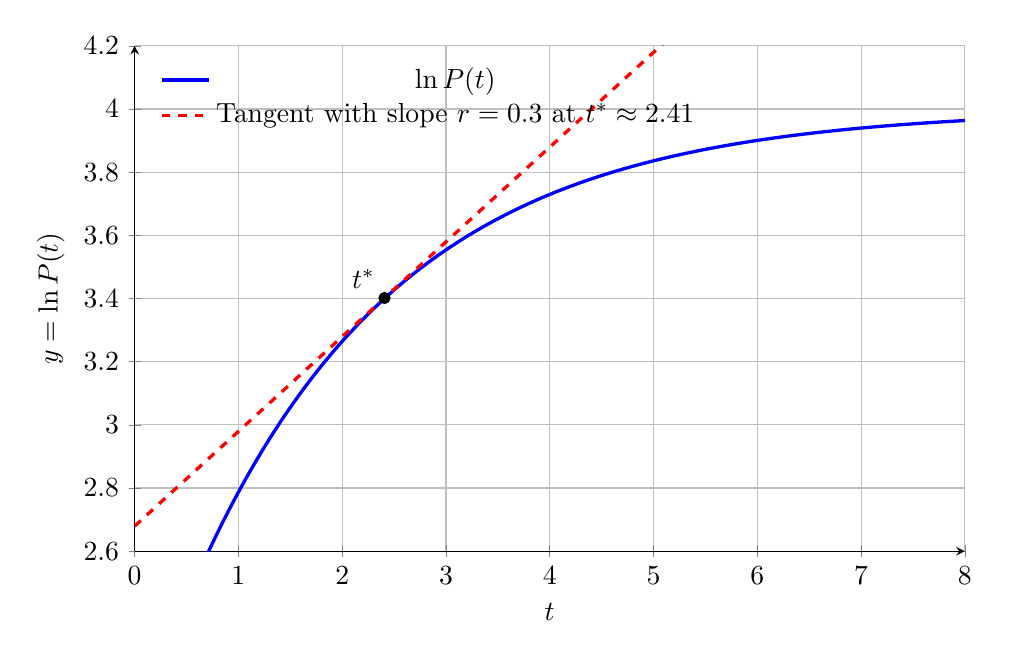
\begin{tikzpicture}
\begin{axis}[
  width=\textwidth, height=8cm,
  xmin=0, xmax=8,
  ymin=2.6, ymax=4.2,
  axis lines=left,
  xlabel={$t$}, ylabel={$y=\ln P(t)$},
  legend style={at={(0.02,0.98)},anchor=north west, draw=none, fill=none},
  domain=0:8, samples=400, grid=both
]
% Choose a concave ln P(t): y = 4 - 2 e^{-0.5 t}
\addplot[very thick, blue] {4 - 2*exp(-0.5*x)};
\addlegendentry{$\ln P(t)$}
% Parameters for tangent construction:
% r = 0.3, t* = (1/0.5)*ln(1/0.3) ≈ 2.408, y* = 4 - 2 e^{-0.5 t*} ≈ 3.4016
\addplot[very thick, red, dashed, domain=0:8] {3.4016 + 0.3*(x - 2.408)};
\addlegendentry{Tangent with slope $r=0.3$ at $t^\ast\approx2.41$}
\addplot[only marks, mark=*, mark size=2pt, black] coordinates {(2.408,3.4016)};
\draw (axis cs:2.408,3.4016) node[anchor=south east] {$t^\ast$};
\end{axis}
\end{tikzpicture}
\caption{Optimal timing condition: choose $t^\ast$ where the slope of $\ln P(t)$ equals the discount rate $r$.}
\label{fig:optimal-timing}
\end{figure}


\begin{figure}[ht]
\centering
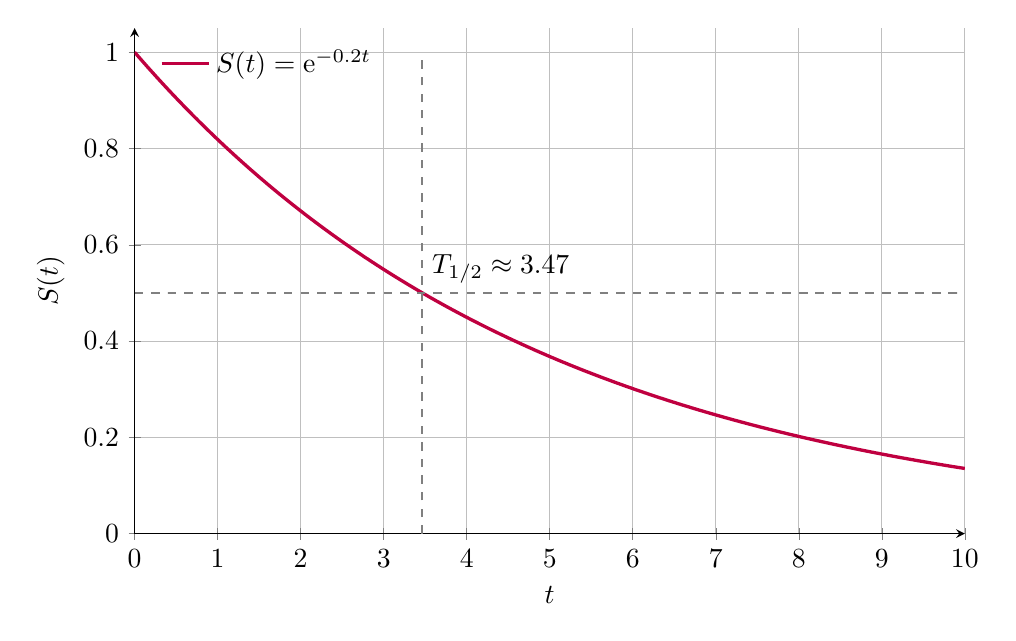
\begin{tikzpicture}
\begin{axis}[
  width=\textwidth, height=8cm,
  xmin=0, xmax=10,
  ymin=0, ymax=1.05,
  axis lines=left,
  xlabel={$t$}, ylabel={$S(t)$},
  legend style={at={(0.02,0.98)},anchor=north west, draw=none, fill=none},
  domain=0:10, samples=400, grid=both
]
% S(t) = e^{-delta t}, delta=0.2
\addplot[very thick, purple] {exp(-0.2*x)};
\addlegendentry{$S(t)=\mathrm{e}^{-0.2 t}$}
% Half-life lines: T_{1/2} = ln(2)/0.2 ≈ 3.466
\addplot[thick, gray, dashed, domain=0:10] {0.5};
\addplot[thick, gray, dashed] coordinates {(3.466,0) (3.466,1)};
\draw (axis cs:3.466,0.5) node[anchor=south west] {$T_{1/2}\approx 3.47$};
\end{axis}
\end{tikzpicture}
\caption{Exponential decay with half-life $T_{1/2}=\ln 2/\delta$.}
\label{fig:half-life}
\end{figure}

\newpage



\section*{References}
\begin{itemize}[leftmargin=1.2em]
\item Simon \& Blume, \emph{Mathematics for Economists}, ch.\ on exponential/log functions and elasticities.
\item Sydsæter \& Hammond (with Strøm \& Carvajal), \emph{Essential Mathematics for Economic Analysis}, sections on logs/exponentials, continuous compounding, and growth accounting.
\end{itemize}


\end{document}
